\section{Auswertung}
\label{sec:Auswertung}

\subsection{Vorbereitung}

Die Größen Ordnungszahl $Z$, Literaturwert der
K-Kante $E_\text{K}^\text{Lit}$, der zugehörige Glanzwinkel 
$\theta_\text{glanz}^\text{Lit}$ und die Abschirmkonstante 
$\sigma_\text{K}$ verschiedener Elemente sind in Tabelle 
\ref{tab:literatur} aufgelistet.

\begin{table}
  \centering
  \caption{Literaturwerte und daraus errechnete Größen verschiedener Elemente}
  \label{tab:literatur}
  \sisetup{table-format=2.1}
  \begin{tabular}{c c c c c}
  \toprule
  $ $ & $Z$ & $E_\text{K}^\text{Lit} \,/\, \si{\kilo\eV}$
  & $\theta_\text{glanz}^\text{Lit} \,/\, \si{\degree}$ & 
  $\sigma_\text{k}$\\
  \midrule 
  Cu & 29 & 08,98 & 20,05 & 3,30 \\
  Zn & 30 & 09,65 & 18,60 & 3,36 \\
  Ge & 32 & 11,10 & 16,10 & 3,43 \\
  Br & 35 & 13,47 & 13,22 & 3,53 \\
  Rb & 37 & 15,19 & 11,69 & 3,58 \\
  Sr & 38 & 16,10 & 11,03 & 3,60 \\
  Zr & 40 & 18,00 & 09,85 & 3,62 \\
  Nb & 41 & 18,99 & 09,33 & 3,63 \\
  Au & 79 & 80,77 & 02,18 & 1,94 \\
  \bottomrule
  \end{tabular}
  \end{table}

Dabei ergibt sich der Glanzwinkel

  \begin{equation}
    \theta_\text{glanz} = \text{arcsin}\left(\frac{h \cdot c}{E \cdot 2d}\right)
    \label{eqn:theta}
  \end{equation}

  durch die Umstellung der Gleichung \eqref{eqn:Bragg} und durch Einsetzen 
  des Ausdrucks $\lambda = \frac{h \cdot c}{E}$. Weiterhin beträgt die Gitterkonstante
  des Kristalls $d_\text{LiF} = \SI{201.4}{\pico\meter}$.

  Die Abschirmkonstante $\sigma_\text{K}$ ergibt sich für die K-Schale aus Gleichung
  \eqref{eqn:std} durch Einsetzen des Ausdrucks $z_\text{eff} = z -\sigma$ und durch 
  Umstellung zu 

  \begin{equation}
    \sigma_\text{K} = z - \sqrt{\frac{E_n}{R_{\infty}}} \; .
    \label{eqn:sigma}
  \end{equation}

  Weiterhin sind zur Überprüfung der Absorption die folgeneden Werte für Kupfer 
  ermittelt worden:

  \begin{align*}
    \text{Für } K_\alpha \text{ : } E_{K_\alpha} &= \SI{8.046}{\kilo\eV}, \\
    \text{Für } K_\beta \text{ : } E_{K_\beta} &= \SI{8.904}{\kilo\eV} \\
    \theta_{K_\alpha} &= \SI{22.49}{\degree}, \\
    \theta_{K_\beta} &= \SI{20.22}{\degree} \: .
 \end{align*}




  %https://wissen.science-and-fun.de/tabellen-fur-spektroskopiker/wellenlaengen-und-anregungsenergien-von-k-und-l-absorptionskanten/





\subsection{Überprüfung der Bragg Bedingung}

Nach der Braggbedingung ist zu erwarten, dass das gemessene Intensitätsmaximum
für einen bestimmten Glanzwinkel auftritt. 
Dies wird durch Abbildung \ref{fig:plot1} verifiziert. In jener ist eindeutig ein Maximum 
mit etwa $310$ Impulsen bei $\SI{27.25}{\degree}$ zu erkennen.

\begin{figure}[H]!
  \centering
  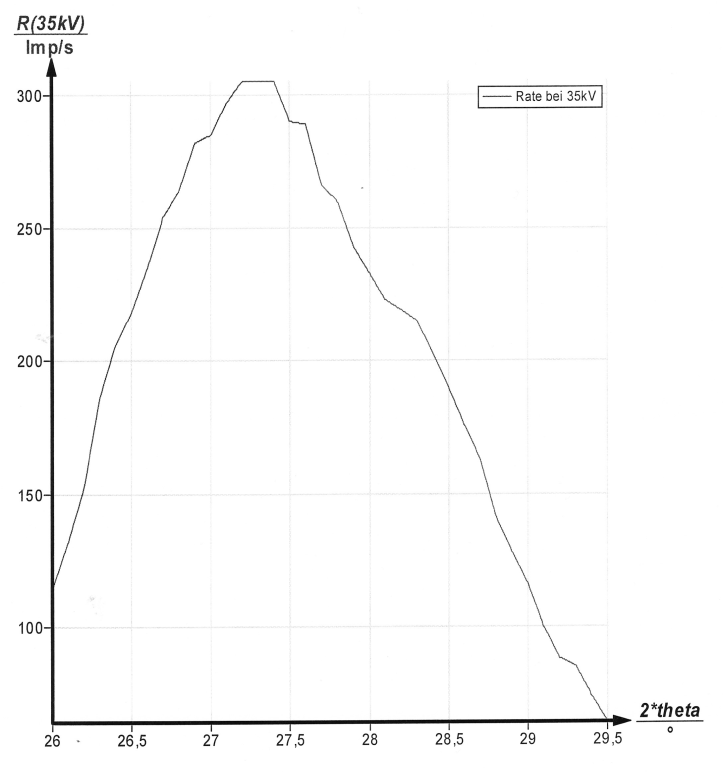
\includegraphics[scale=0.3]{content/bild1.png}
  \caption{Winkelabhängigkeit der Intensitätsmessung}
  \label{fig:plot1}
\end{figure}

\subsection{Das Emissionsspektrum einer Kupferröntgenröhre}

Das gemessene Emissionsspektrum der Kupferanode ist in Abbildung \ref{fig:plot2} abgebildet.
In dieser sind mit zunehmendem Winkel gut der Grenzwinkel bei etwa $\SI{5}{\degree}$,
der Bremsberg im Bereich von $\SI{5}{\degree}$ bis $\SI{19}{\degree}$, die 
$K_\beta$-Kante bei etwa $\SI{20}{\degree}$ und die $K_\alpha$-Kante bei 
etwa $\SI{22.5}{\degree}$ zu erkennen. 

Nach Formel \eqref{eqn:Bragg} mit $n = 1$ ergeben sich aus dem gemessenen Grenzwinkel die 
minimale Wellenlänge $\lambda_\text{min} = \SI{35.106}{\pico\meter}$ und maximale
Energie $E_\text{max} = \SI{5.658}{\femto\joule} = \SI{35.316}{\kilo\eV}$.
Die nach Formel \eqref{eqn:lambda} errechneten Werte sind hingegen hingegen
$\lambda_\text{min} = \SI{35.424}{\pico\meter}$ und 
$E_\text{max} = \SI{5.608}{\femto\joule} = \SI{35}{\kilo\eV}$.
Dabei weichen die gemessenen Werte um $\SI{0.9}{\percent}$ von den errechneten ab.

Die Halbwärtsbreiten betragen für die $K_\alpha$-Kante bei $2100$ Impulsen
etwa $\Delta \theta_\alpha = \SI{0.5}{\degree}$ und die $K_\beta$-Kante bei $600$ Impulsen
etwa $\Delta \theta_\beta = \SI{0.7}{\degree}$.
Mithilfe der Formel

\begin{equation}
  \Delta E = \frac{h \cdot c}{2d \cdot \text{sin}\left(\Delta \theta \right)}
\end{equation}

ergeben sich die Energiedifferenzen 

\begin{align*}
  \Delta E_\alpha &= \SI{0.252}{\kilo\eV} \\
  \Delta E_\beta &= \SI{0.353}{\kilo\eV}  \; .
\end{align*}

\begin{figure}[H]!
  \centering
  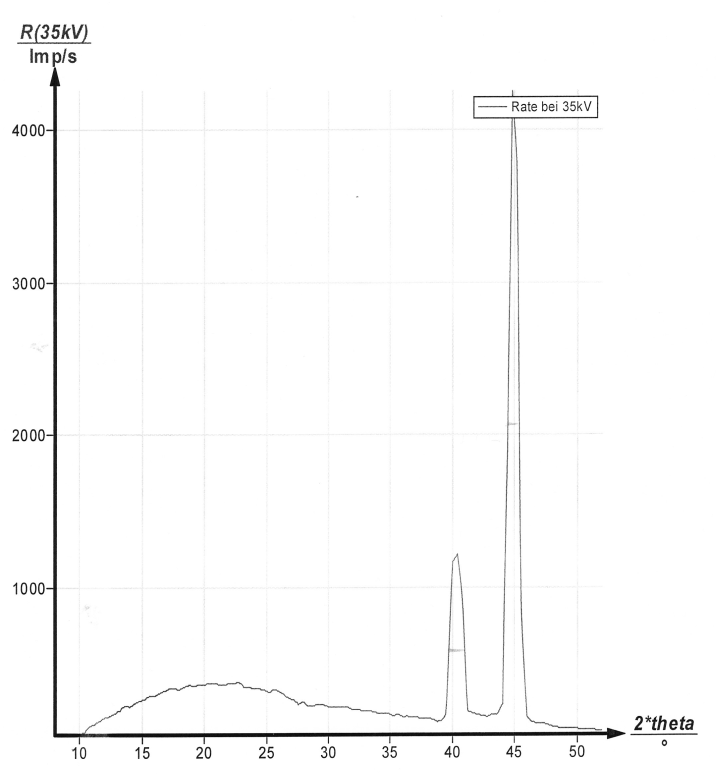
\includegraphics[scale=0.3]{content/bild2.png}
  \caption{Emissionsspektrum der Kupferanode}
  \label{fig:plot2}
\end{figure}

Das Auflösungsvermögen der Apparatur ergibt sich dabei als der Mittelwert der 
Energiedifferenzen $ x = \SI{0.3025 +- 0.0505}{\kilo\eV}$.

Für die K-Linien ergeben sich aus den abgelesenen Glanzwinkeln 

\begin{align*}
  \theta_{K_\alpha} &= \SI{22.5}{\degree} \\
  \theta_{K_\beta} &= \SI{20}{\degree}
\end{align*}

die Energien 

\begin{align*}
E_{K_\alpha} &= \SI{8.043}{\kilo\eV} \\
E_{K_\beta} &= \SI{9.000}{\kilo\eV} 
\end{align*}.

Aus Gleichung \eqref{eqn:sigma} lässt sich mit der Energie der $K_\beta$-Schale
die erste Abschirmkonstante als $\sigma_1 = 3.275$ berechnen. Aus der Gleichung
\eqref{eqn:std} ergibt sich die Beziehung

\begin{equation}
  E_{K_\alpha} = R_\infty (z - \sigma_1)^2 \frac{1}{1^2} - R_\infty (z - \sigma_2)^2 \frac{1}{2^2}  \; \text{,}
\end{equation}

die sich zu

\begin{equation}
  \sigma_2 = z - 2 \sqrt{\frac{R_\infty (z - \sigma_1)^2 - E_\alpha}{R_\infty}}
\end{equation}

umstellen lässt, sodass sich die zweite Abschirmkonstante $\sigma_1 = 12.223$ bestimmen lässt.

\subsection{Die Absorptionsspektren verschiedener Stoffe}

\subsubsection{Zink}

In Abbildung \ref{fig:plot3} ist das gemessene Absorptionsspektrum von Zink abgebildet.
Die K-Kante ist bei etwa $\SI{18.5}{\degree}$ lokalisiert. Durch Umstellung 
der Gleichung \eqref{eqn:theta} wird die Absorptionssenergie als 
$ E_\text{Zn, K} = \SI{9.701}{\kilo\eV}$ mit einer relativen Abweichung
zum theoretischen Wert von $\SI{0.53}{\percent}$ bestimmt. Die Abschirmkonstante
berechnet sich nach Gleichung \eqref{eqn:sigma} zu $\sigma_\text{Zn, K} = 3.293$
mit einer relativen Abweichung von $\SI{2.0}{\percent}$.

\begin{figure}[H]!
  \centering
  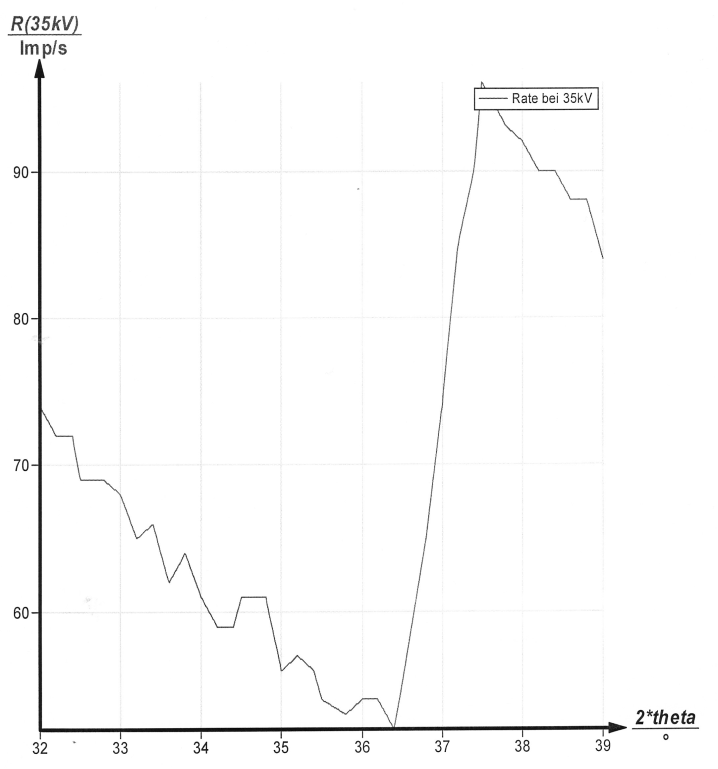
\includegraphics[scale=0.3]{content/bild7.png}
  \caption{Absorptionsspektrum von Zink}
  \label{fig:plot3}
\end{figure}

\subsubsection{Brom}

Das Absorptionsspektrum von Brom ist in Abbildung \ref{fig:plot4} zu sehen.
Auch hier ist deutlich eine K-Kante bei etwa $\SI{13.0}{\degree}$ zu erkennen.
Es ergeben sich nach den Gleichungen \eqref{eqn:theta} und \eqref{eqn:sigma}
die Absorptionssenergie $ E_\text{Br, K} = \SI{13.683}{\kilo\eV}$ mit einer 
relativen Abweichung von $\SI{1.58}{\percent}$ zum Literaturwert und die 
Absorptionskonstante $\sigma_\text{Br, K} = 3.281$ mit einer relativen
Abweichung von $\SI{7.05}{\percent}$.

\begin{figure}[H]!
  \centering
  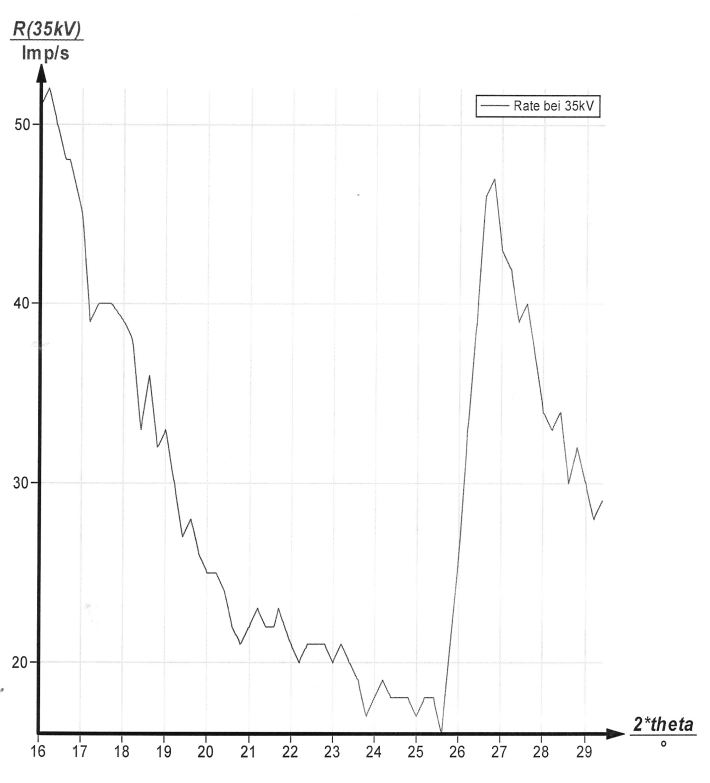
\includegraphics[scale=0.3]{content/bild6.png}
  \caption{Absorptionsspektrum von Brom}
  \label{fig:plot4}
\end{figure}

\subsubsection{Strontium}

Abbildung \ref{fig:plot5} zeigt das Absorptionsspektrum von Strontium mit einer 
K-Kante bei etwa $\SI{10.8}{\degree}$ mit der nach Formel \eqref{eqn:theta}
zugehörigen Absorptionssenergie $ E_\text{Sr, K} = \SI{16.427}{\kilo\eV}$,
die um $\SI{2.03}{\percent}$ vom Theoriewert abweicht. Die sich nach Formel 
\eqref{eqn:sigma} ergebende Absorptionskonstante $\sigma_\text{Sr, K} = 3.246$
weicht um $\SI{9.83}{\percent}$ ab.

\begin{figure}[H]!
  \centering
  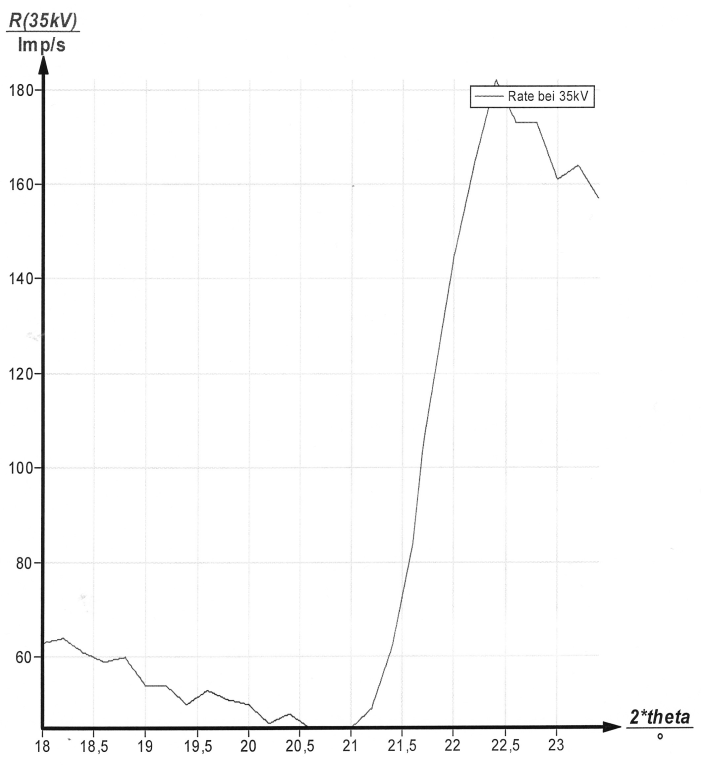
\includegraphics[scale=0.3]{content/bild5.png}
  \caption{Absorptionsspektrum von Strontium}
  \label{fig:plot5}
\end{figure}

\subsubsection{Zirkonium}

Das Absorptionsspektrum von Zirkonium ist in Abbildung \ref{fig:plot6} dargestellt.
Bei einem Winkel von $\SI{9,65}{\degree}$ ist die K-Kante zu erkennen. Die
Absorptionssenergie von $E_\text{Zr, K} = \SI{18.362}{\kilo\eV}$ weicht
um $\SI{2.01}{\percent}$ relativ ab. Nach Formel \eqref{eqn:sigma} ergibt 
sich die Abschirmkonstante $\sigma_\text{Sr, K} = 3.256$, die um 
$\SI{10.06}{\percent}$ von ihrem Theoriewert abweicht.

\begin{figure}[H]!
  \centering
  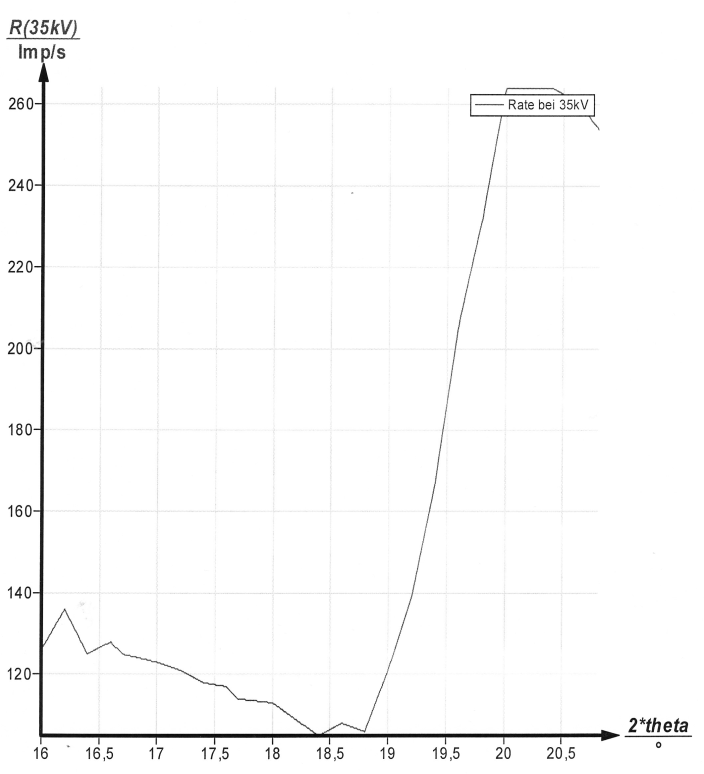
\includegraphics[scale=0.3]{content/bild4.png}
  \caption{Absorptionsspektrum von Zirkonium}
  \label{fig:plot6}
\end{figure}

\subsection{Mosleysches Gesetz}

Die Quadratwurzeln der Absorptionsenergien verschiedener Elemente
sind in Abbildung \ref{fig:plotx} gegen die jeweilige Ordnungszahl aufgetragen.

\begin{figure}[H]!
  \centering
  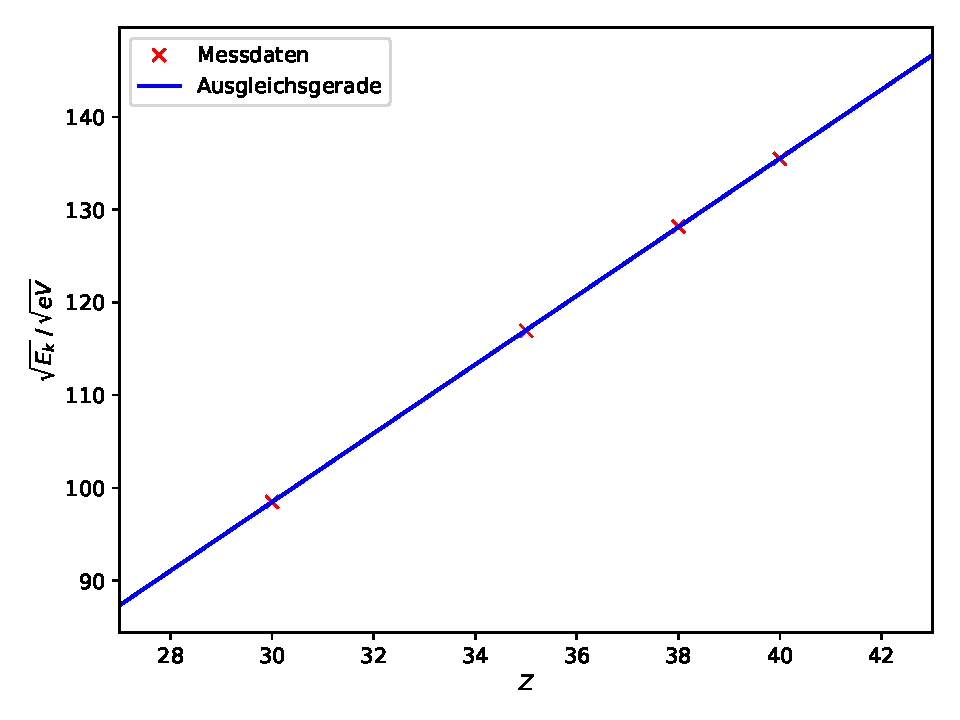
\includegraphics[scale=0.7]{content/plot1.pdf}
  \caption{Die Qudratwurzeln der Absorptionsenergien verschiedener Elemente}
  \label{fig:plotx}
\end{figure}

Nach einer linearen Regression mittels python ergeben sich die
Regressionsparameter als

\begin{align*}
  a &= \SI{3.705 +- 0.005}{\per \kilo \eV \tothe{1/2}} \\
  b &= \SI{-12.663 +- 0.192}{\kilo \eV \tothe{1/2}}
\end{align*}

Nach Gleichung \eqref{eqn:std} ist die Quadratwurzel der Rydberg-Energie
$\sqrt{R_\infty}$ die Geradensteigung. Folglich beträgt die experimentell
bestimmte Rydbergenergie $R_\infty = \SI{13.73}{\eV}$ und weicht von ihrem
Theoriewert um etwa $\SI{0.96}{\percent}$ ab.

\subsection{Die L-Kanten des Absorptionsspektrums von Gold}

In Abbildung \ref{fig:plot7} ist das gemessene Absorptionsspektrum von Gold abgebildet.
Die L-Kante sind bei etwa $\SI{13.5}{\degree}$ und $\SI{15.0}{\degree}$ lokalisiert.
Durch Umstellung der Gleichung \eqref{eqn:theta} werden die Absorptionssenergien 
$ E_1 = \SI{13.185}{\kilo\eV}$ und $ E_2 = \SI{11.893}{\kilo\eV}$ bestimmt.
Die Energiedifferenz beträgt also $\Delta E_\text{Au, L} = \SI{1.292}{\kilo\eV}$.
Die Abschirmkonstante berechnet sich nach Gleichung \eqref{eqn:crap} zu 
$\sigma_\text{Au, L} = 9.127$ mit der Feinstrukturkonstante
$\alpha = 0.0072974$.

\begin{figure}[H]!
  \centering
  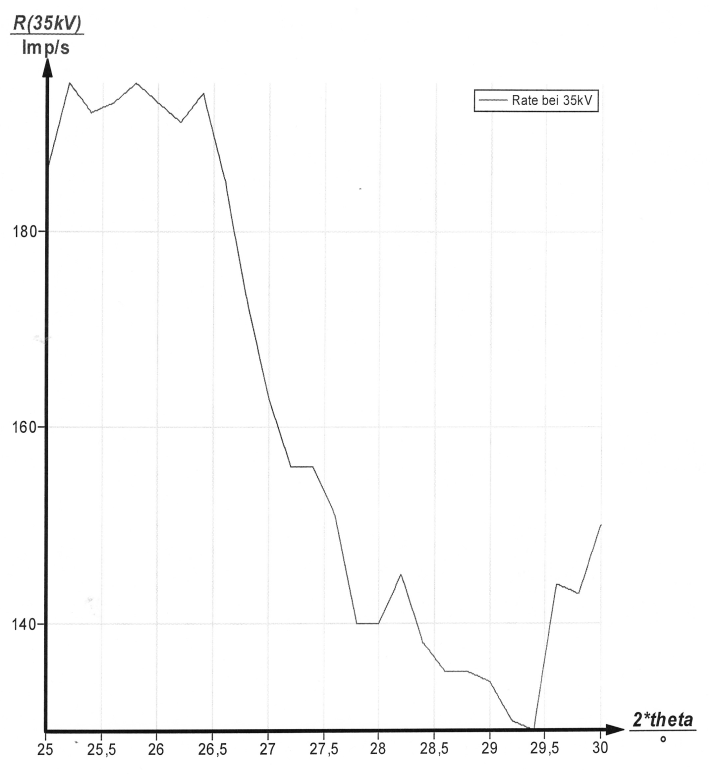
\includegraphics[scale=0.3]{content/bild3.png}
  \caption{Absorptionsspektrum von Gold}
  \label{fig:plot7}
\end{figure}







